% Chapter 2



\chapter{Geometric Compensation Technique} % Main chapter title$
\label{Chapter2} 
It is shown in the previous chapter that the idea of implementing a broadband antenna using a linearly graded dielectric was successful in coupling the leaky-wave radiation into free-space. However, it has high sidelobe levels and the main beam direction is inconsistent over broad bandwidth. In the second approach to the design of the antenna, conformal transformation has been employed to transform a region with a convex upper interface to a rectangular domain. It is demonstrated in this chapter that the phase distribution at the interface of an optically transformed medium is not identical from the initial domain, which leads to undesired antenna performance. This chapter is dedicated to developing a technique that can eliminate the phase-deviations to improve the antenna performance. The technique is used to design the fixed-beam leaky-wave antenna in the following chapter.
%A numerical approach is followed by solving Laplace's equation that defines the rules of coordinate transformations between two domains. %%%%%%%%%%%%%%%%%%%%%%%%%%%%%%%%%%%%%%

%%%%%%%%%%%%%%%%%%%%%%%%%%%%%%%%%%%%%%%%%%%%%%%%%%%%%%%%%%%%%%%%%%%%
\section{Numerical conformal transformation}
Transformation electromagnetics allows controlling the propagation of electromagnetic waves in a medium by engineering its constituent parameters. Conformal transformation is a special category of transformation optics that reduces material complexity of the resultant medium by employing isotropic inhomogeneous graded index structures.

\subsection{Linking to the antenna design}
In the introductory section \ref{sec:TO}, it has been demonstrated how conformal transformation can be employed to transform a curved geometry into an electromagnetically equivalent rectangular domain. A Jacobian matrix $\Lambda$ relates the material parameters of the intial region into the transformed region as demonstrated in Eqs. \ref{eq:transconda} and \ref{eq:transcondb}. This thesis denotes the initial geometry as the source domain in $(x$,$y)$ coordinates and the transformed geometry as the target domain in $(u$,$v)$ coordinate. %Hence, the transformation process would result in a rectangular geometry as the target domain described by $(u,v)$ coordinate. 

The conformal transformation was executed numerically using COMSOL Multiphysics \cite{Ma2010}. The numerical approach is implemented by solving Laplace's equation to define the rules of coordinate mapping between two domains. The dielectric permittivity of transformed medium consists of two-dimensional variations. The technique is used in section \ref{sourtotargettrans} for developing the geometric compensation technique. Therefore, the numerical transformation was restricted to two-dimensional (2D) domain.

\subsection{Validation of simulations}
\label{App:TO}

The numerical transformation electromagnetics for the development of the geometric compensation technique has been carried out using COMSOL Multiphysics. Prior to applying the technique for designing the antenna, the numerical process was validated by performing conformal transformation between arbitrary 2D geometries, as demonstrated in Fig. \ref{fig:TOvalidation}. The geometry $ABCD$ filled with uniform dielectric material in the initial domain was transformed into the isotropic inhomogeneous dielectric with a geometry $A'B'C'D'$ in the transformed domain.

\begin{figure} [t]
\pgfplotsset{compat=1.5,
scale=.1,
tick label style={font=\small},
label style={font=\small},
legend style={font=\small},
width=7.5cm,
height=4.64cm,
% tick style={thick}
}
\begin{center}
  \hspace*{\fill}
\includestandalone[width=0.28\textwidth]{Figures/Chapter3/TO_validation/fig_geom1_standalone}
\put(-117,-10){\footnotesize $A$}
\put(-117,20){\footnotesize $B$}
\put(-5,-10){\footnotesize $D$}
\put(-20,47){\footnotesize $C$}
\put(-90,-23){\footnotesize Initial domain ($\mathrm{w}$)}
\hspace{.5cm}
  \hspace*{\fill}
\includestandalone[width=0.28\textwidth]{Figures/Chapter3/TO_validation/fig_geom3_standalone}
\put(-113,-10){\footnotesize $a$}
\put(-113,31){\footnotesize $b$}
\put(-5,-10){\footnotesize $c$}
\put(-7,31){\footnotesize $d$}
\put(-104,-23){\footnotesize Intermediate domain ($\mathrm{r}$)}
  \hspace*{\fill}
\includestandalone[width=0.28\textwidth]{Figures/Chapter3/TO_validation/fig_geom2_standalone}
\put(-114,-10){\footnotesize $A'$}
\put(-114,31){\footnotesize $B'$}
\put(-7,-10){\footnotesize $D'$}
\put(-20,31){\footnotesize $C'$}
\put(-105,-23){\footnotesize Transformed domain ($\mathrm{t}$)}
  \hspace*{\fill}
    \end{center}
 \caption[Validation of numerical transformation electromagnetics by transforming uniform dielectric into a region filled with isotropic inhomogeneous dielectric medium.]{Optical transformation from region $ABCD$ filled with uniform dielectric material into an isotropic inhomogeneous dielectric medium $A'B'C'D'$. For the validation process, the domains were excited with a point source at points $A$ and $A'$.}
\label{fig:TOvalidation}
\end{figure}

Conformal transformation can only take place between two media provided that one of the media is rectangular \cite{Burokur2016}. However, the geometries in Fig. \ref{fig:TOvalidation} do not fulfill the criteria. Therefore, the transformation was performed through an intermediate rectangular geometry. In other words, the transformation $\mathrm{t} \longrightarrow \mathrm{w}$ has to be performed through an intermediate rectangular domain $\mathrm{r}$. In the first step, the initial domain $\mathrm{w}$ is transformed to the intermediate domain $\mathrm{r}$ using transformation equation $\mathrm{r} \longrightarrow \mathrm{w}$, as presented in Fig. \ref{fig:TOvalidation}. The ratio of height to width of the intermediate domain represents the conformal module of the two transformations. In the second step, the transformed domain $\mathrm{t}$ is transformed to the intermediate domain $\mathrm{r}$ using transformation equation $\mathrm{r} \longrightarrow \mathrm{t}$. The conformal module for the both transformations are same. The coordinate grids of the initial and transformed domains are presented in Fig. \ref{fig:TOvalidation2}. The relative permittivity distribution of transformed domain was obtained from the solution of the numerical conformal transformation process. The initial and transformed domains were then excited with a point source at the bottom-left corners ($A$ and $A'$) in order to verify that the two media had identical electromagnetic behavior. The rules of coordinate transformation and transformation optics is valid only inside initial and transformed domains. The transformation equations do not incorporate the interaction of associated domains with external media. In order to ensure validation of the transformation process, it is necessary to eliminate the interaction of the transformation regions $\mathrm{w}$ and $\mathrm{t}$ with free-space. The boundaries were enclosed with a perfect electric conductor (PEC) to neglect the interaction with external media. 
%
\begin{figure}[]
\centering
\noindent
  \hspace*{\fill}
  \mbox{\subfloat[]
        {\begin{overpic}[scale = .37,trim=0 5.2cm 0 5cm,clip]{Figures/Chapter3/TO_validation/Domain1}
    \put(-4,0){\footnotesize $A$}
    \put(-4,10){\footnotesize $B$}
    \put(97.5,0){\footnotesize $D$}
    \put(83,40){\footnotesize $C$}
        \end{overpic}
        
        }}
  \hspace*{\fill}
 \mbox{\subfloat[]
        {\begin{overpic}[scale = .37,trim=0 6cm 0 5cm,clip]{Figures/Chapter3/TO_validation/Domain2}	
    \put(-4,0){\footnotesize $A'$}
    \put(-4,23){\footnotesize $B'$}
    \put(98,0){\footnotesize $D'$}
    \put(88,23){\footnotesize $C'$}
        \end{overpic}
        }}
 \hspace*{\fill}%
\caption[Coordinate grid lines of the transformation shown in Fig. \ref{fig:TOvalidation}.]{(color inline) Coordinate grids during the optical transformation process of the initial and transformed domain of Fig. \ref{fig:TOvalidation}.}
\label{fig:TOvalidation2}
\end{figure}
%

The electromagnetic waves propagates within the media and completely reflects from the PEC boundaries, creating standing waves throughout the domain. The electric field values inside the two media have to be identical at the equivalent points if the transformation is accurate. Arbitrary points in initial domain were selected that are test points over which the fields were compared with equivalent points in the transformed domain. The test point locations in transformed domain that corresponded to the ones in initial domain were determined by applying the coordinate transformation to the test points. The normalized electric field values of the standing waves at the test points for both media are presented in Fig. \ref{fig:TOvalidplot}. The brown lines represents the normalised field values of the standing waves in initial domain while the green line shows the same at equivalent points of transformed domain. The figure shows that the standing waves inside the two media creates identical field values at equivalent test points. 

\begin{figure} [t!]
  \begin{center}
 \begin{tikzpicture}

\begin{axis}[transpose legend,
legend columns=1,
legend style={at={(0.78,1)},anchor=north},
cycle multi list={%
{red,mark={}},
{blue,solid,mark={}},
},
ymin=0,
ymax=1,
xmin=0,
xmax=.6,
xlabel={Horizontal distance in the initial domain $(\lambda_0)$},
ylabel={Normalised Electric field ($V/m$)},
%xtick={0,1,2,3,4,5,6},
%ytick={-1.4612e+03,-730.6029,0,730.6029,1.4612e+03},
%xticklabels={$0$,$1$,$2$,$3$,$4$,$5$,$6$},
%title=Decay of Electric Field along the Single Slot and Slot Array under different dielectrics,
%xticklabel=\empty,
% yticklabel=\empty,
%xlabel={$Wave vector (K_{x}a_{x}/2\pi)$},
%ylabel={$Wave vector (K_{y}a_{y}/2\pi)$},
% extra x ticks={-78.54,78.54},
% extra y ticks={-78.54,78.54},
% extra x tick labels={$-0.0625$,$0.0625$},
% extra y tick labels={$-0.0625$,$0.0625$},
% smooth,
grid=major,
%legend entries={$\epsilon_r = 2$ (single slot),$\epsilon_r = 4$ (single slot),$\epsilon_r = 2$ (slot array),$\epsilon_r = 4$ (slot array)}
legend entries={Medium 1, Medium 2}
];
\addplot [thick, color=dbrown,mark=o, solid] table [col sep=comma] {Figures/Chapter3/TO_validation/xy.csv};

\addplot [thick, color=dgreen, mark=diamond, solid] table [col sep=comma] {Figures/Chapter3/TO_validation/xprimeyprime.csv};

\end{axis}
\end{tikzpicture}
 \end{center}
  \caption[Normalized absolute value of the electric field in the standing waves in initial domain and transformed domain confirming the numerical transformation process.]{(color inline) Normalized absolute value of the electric field in the standing waves in initial domain (brown) and transformed domain (green). The points in the initial domain were arbitrarily selected along the vertical coordinate grid $.14 \lambda_0 $. The test locations in transformed domain corresponding to the equivalent points in initial domain were selected from transformation results.}
\label{fig:TOvalidplot}
\end{figure}

The overlapping lines in Fig. \ref{fig:TOvalidplot} indicates that the fields inside the initial and transformed domains enclosed by PEC boundaries have identical standing wave patterns. Therefore, it can be deduced that both domains are electromagnetically identical.
%%%%%%%%%%%%%%%%%%%%%%%%%%%%%%%%%%%%%%%%%%%%%%%%%%%%%%%%%%%%%%%%%%%%

\section{Geometric compensation technique}

\subsection{Principle}

%previous comments:
In order to achieve a fixed angle of radiation, a linear phase gradient in the target domain is required. This corresponds to a linear phase gradient in the source domain. Since the transformation equations are unknown prior to performing the source-to-target domain transformation, a perturbation approach is required to find a source domain geometry that transforms into a target domain having the required linear phase. The idea is demonstrated in Fig. \ref{fig:diagram_phasecomp}. The perturbation approach, named the \textit{geometric compensation} technique, begins by choosing a linear phase gradient (red line) in the source domain and obtaining a geometric path $s$ that possesses that phase gradient. This path then defines the upper interface of the target domain (see Fig. \ref{fig:diagram_phasecomp}a). Using conformal transformation optics, the source domain geometry is mapped into a rectangular target domain. Due to coordinate stretching, the phase distribution along the upper interface of the target domain becomes a function of $u$, as shown by the red line in see Fig. \ref{fig:diagram_phasecomp}b. However, a linear phase is required in the target domain to achieve a fixed-beam radiation. In order to fix this discrepancy in linear phase, the phase errors are determined and transformed back into the source domain using the transformation equations. The inverse-transformed phase profile, shown by the blue line in Fig. \ref{fig:diagram_phasecomp}c, is used to achieve an altered geometry $s'$. Further transformations are performed to find the required linear phase in the target domain (see Fig. \ref{fig:diagram_phasecomp}d). The procedure is used in the following chapter to achieve broadband fixed-beam performance from a leaky-wave antenna. Before applying the technique in antenna design, each step of the technique is demonstrated below using a point source excitation. 
\begin{figure} [p!]
\centering
  \noindent

   \begin{overpic}[trim={0cm 0.0cm 0cm 0cm},clip,scale=0.55, keepaspectratio=true]{Figures/Chapter3/fig_compensation/phase_correction}
        \put(65,83){\footnotesize \rotatebox{90}{Source Domain}}
        \put(65,57){\footnotesize \rotatebox{90}{Target Domain}}
        \put(65,32){\footnotesize \rotatebox{90}{Source Domain}}
        \put(65,6){\footnotesize \rotatebox{90}{Target Domain}}
	\end{overpic}

  \caption[A diagram illustrating the process of geometric compensation compensation.]{A diagram illustrating the process of geometric compensation compensation. The source domain is represented by $(x$,$y)$ coordinate, while the target domain is in $(u$,$v)$ coordinate. The left columns presents the phase distributions along the upper interface of the geometries to their right. The compensated and uncompensated geometries are presented by red and blue lines, respectively.}
\label{fig:diagram_phasecomp}
\end{figure}


\subsection{Linear phase gradient at the radiating interface}
The first step of the technique is to determine a path through the source domain along which the fields have a linear phase gradient. The geometry shown in the source domain in Fig. \ref{fig:pointphase} comprises of a curved interface along which the phase fronts interact with a linear profile. The angle of the coupled radiation is $\theta_{\mathrm{rad}}$ is related to the phase gradient along the upper interface by the following equation:
 
%
\begin{equation} \label{eq:linphase2}
\dfrac{d\phi}{ds} = k_0 \sin\theta_{\mathrm{rad}}  = \textrm{constant}
\end{equation}
%
where $k_0$ is the free-space wave number and $ds$ is the change in arc length of the boundary of the air interface which is a function of the space. For a straight path $s$, a linear phase gradient in Eq. \ref{eq:linphase2} would produce a radiated beam at an angle of $\theta_{\mathrm{rad}}$. We wish to find the path in the source domain that corresponds to the same gradient so that it can be transformed into the rectangular target domain.

\begin{figure} [t!]
\centering
  \noindent

   \begin{overpic}[trim={0cm 0.0cm 0cm 0cm},clip,scale=0.6, keepaspectratio=true]{Figures/Chapter2/fig_point_phasegrad/point_phasegrad}
	\put(34,42){\footnotesize $\theta_{\mathrm{rad}}$}
	\put(80,32){\footnotesize $\theta_{\mathrm{rad}}$}
	\put(8,-2){\footnotesize Source domain}
	\put(69,-2){\footnotesize Target domain}
	\end{overpic}

  \caption[The initial and target domain geometries excited with a point source.]{The initial and target domain geometries excited with a point source. The initial domain consists of uniform dielectric material, while the rectangular target domain geometry contains graded index materials. The dotted lines represent phase fronts of the radiated wave. It is expected that both media will have identical phase profile at the upper-interface, leading to the same angle of radiation from broadside.}
\label{fig:pointphase}
\end{figure}
%%%%%%%%%%%%%%%%%%%%%%%%%%%%%%%%%%%%%%%%%%%%%%%%%%%%%%%%%%%%%%%%%%%%%%%
\subsection{Determining the source domain geometry} \label{detsourcedom}
The initial geometry in the source domain consists of uniform dielectric, selected such that the source-generated radiation meets the interface with a linear phase delay. The curvature of upper interface of the source domain geometry determines the radiation angle in the target domain. The shape of the source domain geometry is obtained from a linear phase gradient. The change of linear phase with respect to space is equal to a constant, which is a function of radiation angle $\theta_{\mathrm{rad}}$. The governing equation is given by:
%
\begin{equation} \label{eq:lingrad}
    \mathbf{\nabla\phi} \cdot \hat{\mathbf{s}} = \dfrac{d\phi}{ds}
\end{equation}
%
where $\mathbf{\nabla\phi}$ is the phase gradient and $\hat{\mathbf{s}}$ refers to the unit vector tangent to the boundary. $\mathbf{\nabla\phi}$ is given by:
%
\begin{equation} \label{eq:phi}
\mathbf{\nabla\phi} = \phi_x \hat{\mathbf{x}} + \phi_y \hat{\mathbf{y}}
\end{equation}
%
where $\phi_x$ and $\phi_y$ are the derivatives of $\phi$ with respect to $x$ and $y$. $d\phi / ds$ in Eq. \ref{eq:lingrad} is a constant related to the free-space wave vector ($k_0$) and radiation angle $\theta_{\mathrm{rad}}$ by Eq. \ref{eq:linphase2}. Equation \ref{eq:lingrad} can be expanded as follows:
%
\begin{equation} 
    |\mathbf{\nabla\phi}| \cdot 1 \cdot \cos(\theta_{s\nabla})= \dfrac{d\phi}{ds}
\end{equation}
%
which leads to the following equation to determine the arc of the source domain geometry:
%
\begin{equation} \label{eq:detsource}
\theta_{s\nabla} =  \arccos\left(\dfrac{|d\phi/ds|}{|\mathbf{\nabla\phi|}}\right)
\end{equation}
%
\begin{figure} [t!]
\centering
  \noindent
%
   \begin{overpic}[trim={0cm 0.0cm 0cm 0cm},clip,scale=0.6, keepaspectratio=true]{Figures/Chapter3/fig_compensation/choosing_s}
      %  \put(65,83){\footnotesize \rotatebox{90}{Source Domain}}
      %  \put(65,57){\footnotesize \rotatebox{90}{Target Domain}}
      %  \put(65,32){\footnotesize \rotatebox{90}{Source Domain}}
      %  \put(65,6){\footnotesize \rotatebox{90}{Target Domain}}
	\end{overpic}
%
  \caption[A diagram showing the process of choosing a geometry in source domain in $(x$,$y)$ coordinate.]{A diagram showing the process of choosing a geometry in the source domain in $(x$,$y)$ coordinate.}
\label{fig:choosing_s}
\end{figure}
%
where $\cos(\theta_{s\nabla})$ is the angle that the upper boundary forms with the phase gradient. From Fig \ref{fig:choosing_s}, the angle of the upper boundary arc (blue line) with respect to $x$ axis is denoted as $\theta_s$ and represented as:
\begin{equation} \label{eq:theta_s}
\theta_s = \theta_{-\nabla} - \theta_{s\nabla}
\end{equation}
where, $\theta_{-\nabla}$ is the angle of the negative gradient of phase with respect to $x$ axis and $\theta_{s\nabla}$ is the angle between the arc and negative gradient. $\theta_{-\nabla}$ can be obtained from the argument of $\mathbf{\nabla\phi}$ in Eq. \ref{eq:phi} and expressed as:
%
\begin{subequations} \label{eq:nalba}
\begin{align}
\theta_{-\nabla}  & = \pi + \theta_{\nabla} \\
\theta_{\nabla}  &= \arctan \left( \dfrac{\phi_y}{\phi_x} \right) 
\end{align}
\end{subequations}
From Eqs. \ref{eq:theta_s}, \ref{eq:detsource} and \ref{eq:nalba}, the final expression for determining the curve by satisfying the following equation:
%
\begin{equation} \label{eq:comp1}
\theta_s =  \pi + \arctan \left( \dfrac{\phi_y}{\phi_x} \right) - \arccos\left(\dfrac{|d\phi/ds|}{|\mathbf{\nabla\phi|}}\right)
\end{equation}
%
%
\begin{figure} [t!]
\centering
  \noindent

   \begin{overpic}[trim={0cm 0.0cm 0cm 0cm},clip,scale=0.4, keepaspectratio=true]{Figures/Chapter2/fig_phasecompensation/simulationdomain}
   		\put(-20,10){\vector(2,0){10}}
   		\put(-20,10){\vector(0,2){10}}
   		\put(-10,11){\footnotesize $x$}
   		\put(-20,21.5){\footnotesize $y$}


	\end{overpic}

  \caption[Diagram of the simulation domain used in the primary step of the geometric compensation technique.]{Diagram of the simulation domain used in the primary step of the geometric compensation technique. A uniform dielectric halfspace has been excited with a point source in the center. To simulated the infinite dielectric halfspace, the boundaries were eliminated with PML. Effective simulation domain was reduced by using PMC symmetry planes. The dark grey region is the simulation domain that was actually simulated.}
\label{fig:pointdomain}
\end{figure}
%
\begin{figure}[t!]
\centering
\noindent
\hspace*{\fill}%
  \mbox{\subfloat[]
        {\begin{overpic}[scale=.5,trim=0cm .2cm .2cm 1cm,clip]{Figures/Chapter2/fig_phasecompensation/Phaseplot3.png}
%	\put(-40,7){\footnotesize Point source}
%	\put(-8,8){\vector(1,0){10}}
%	\put(-40,39){\footnotesize Desired upper}
%	\put(-36,33){\footnotesize boundary}
%	\put(-6,42){\vector(1,0){8}}
%	\linethickness{.7mm}
%	\put(10,83){\line(2,0){25}}
%	\put(20,85){\footnotesize $\lambda_0$}
	\end{overpic}
        }}
\hspace*{\fill}%
\pgfplotsset{compat=1.5,
width=5.2cm,
height=5.2cm,
tick label style={font=\small},
label style={font=\small},
legend style={font=\small},
% tick style={thick}
}
	\mbox{\subfloat[]
        {\begin{tikzpicture}

\begin{axis}[transpose legend,
legend columns=1,
legend style={at={(0.78,1)},anchor=north},
cycle multi list={%
{red,mark={}},
{blue,solid,mark={}},
},
ymin=-26,
ymax=-14,
xmin=0,
xmax=3,
xlabel={Arc Length ($\lambda_0$)},
ylabel={Unwrapped phase (degrees)},
xtick={0,1,2,3},
%ytick={-1.4612e+03,-730.6029,0,730.6029,1.4612e+03},
xticklabels={$0$,$1$,$2$,$3$,$4$,$5$,$6$,$7$, $8$},
%title=Decay of Electric Field along the Single Slot and Slot Array under different dielectrics,
%xticklabel=\empty,
% yticklabel=\empty,
%xlabel={$Wave vector (K_{x}a_{x}/2\pi)$},
%ylabel={$Wave vector (K_{y}a_{y}/2\pi)$},
% extra x ticks={-78.54,78.54},
% extra y ticks={-78.54,78.54},
% extra x tick labels={$-0.0625$,$0.0625$},
% extra y tick labels={$-0.0625$,$0.0625$},
% smooth,
grid=major,
%legend entries={$\epsilon_r = 2$ (single slot),$\epsilon_r = 4$ (single slot),$\epsilon_r = 2$ (slot array),$\epsilon_r = 4$ (slot array)}
%legend entries={single slot, slot array}
];
\addplot [thick, color=blue,  solid] table [col sep=comma] {Figures/Chapter2/fig_phasecompensation/linphase_point.csv};


\end{axis}
\end{tikzpicture}
        }}
 \hspace*{\fill}%
\caption[Selection of a source domain geometry using a target linear phase profile.]{(color inline) Determination of initial geometry with a point source that leads to $30^\circ$ of radiation in the target domain. The surface plot in (a) represents the unwrapped phase (degrees) of the transverse electric field. The point source generating the fields is located at coordinate point $(0,0)$. The blue curve represents the desired upper interface. The interface is determined by selecting the points that corresponds to the linear phase profile (degrees) in (b).}
\label{fig:inidet}
\end{figure}
%

The upper boundary of the source domain turns out to be convex since it corresponds to the phase of field being radiated obliquely leaving the medium at a fixed angle. Using the curvature equation in Eq. \ref{eq:comp1}, the geometry of the source domain is cropped from a uniform dielectric half-space. Figure \ref{fig:pointdomain} presents the uniform dielectric half-space which is a basis for determining the source domain geometry. The source of uniform dielectric half space is identical to point source of the desired source domain geometry. The idea is to ensure that the source domain geometry (in Fig. \ref{fig:diagram_phasecomp}) and uniform dielectric half space (in Fig. \ref{fig:pointdomain}) possess identical phase distributions since the former is a portion of the later. 
The point source is allowed to radiate into a uniform dielectric halfspace, forming a phase distribution in the medium. Figure \ref{fig:inidet}a shows the selection of the geometry for a radiation of $30^\circ$ in the source domain. Corresponding phase delay along the upper interface is presented in Fig. \ref{fig:inidet}b.) 



%%%%%%%%%%%%%%%%%%%%%%%%%%%%%%%%%%%%%%%%%%%%%%%%%%%%%%%%%%
\subsection{Optically transform the source domain into target domain} \label{sourtotargettrans}
\begin{figure} [t!]
\centering
  \noindent
\hspace*{\fill}%
	\noindent
	\mbox{\subfloat[]{
  \begin{overpic}[trim={0cm 0.0cm 0cm 0cm},clip,scale=0.20, keepaspectratio=true]{Figures/Chapter2/fig_phasecompensation/Compensated_source.png}
				\put(0,50){\footnotesize $A$}
				\put(93,20){\footnotesize $B$}
				\put(0,-2){\footnotesize $C$}
				\put(91,-2){\footnotesize $D$}
				\put(-10,-10){\vector(2,0){20}}
				\put(-10,-10){\vector(0,2){20}}
				\put(14,-12){\footnotesize $x$}
				\put(-10,14){\footnotesize $y$}
	\end{overpic}}}
\hspace*{\fill}%
  \mbox{\subfloat[]{
  \begin{overpic}[trim={0cm 1.5cm 0cm 0cm},clip,scale=0.20, keepaspectratio=true]{Figures/Chapter2/fig_phasecompensation/Compensated_target.png}
			    \put(-2,43){\footnotesize $a$}
				\put(97,43){\footnotesize $b$}
				\put(-2,0){\footnotesize $c$}
				\put(97,0){\footnotesize $d$}
				\put(-10,-10){\vector(2,0){20}}
				\put(-10,-10){\vector(0,2){20}}
				\put(12,-12){\footnotesize $u$}
				\put(-12,14){\footnotesize $v$}
				\put(9,51){\vector(2,0){88}}
				\put(94,51){\vector(-2,0){88}}
				\put(47,54){\footnotesize $L$}
				\put(105,2){\vector(0,2){42}}
				\put(105,44){\vector(0,-2){42}}
				\put(107,21){\footnotesize $H'$}
	\end{overpic}}}
	  \hspace*{\fill}%
    \caption[The initial conformal mapping from a homogeneous source domain to rectangular graded dielectric target domain.]{Conformal mapping from initial homogeneous source domain $ABCD$ in $(x$,$y)$ coordinate (a) to a rectangular graded dielectric target domain $A'B'C'D'$ $(u$,$v)$ coordinate(b).}
\label{fig:pointuncomp}
\end{figure}

Once the geometry in the source domain is obtained, the optical transformation is applied. Consider the transformation $f$ between the source domain in Fig. \ref{fig:pointuncomp}a and the target domain in Fig. \ref{fig:pointuncomp}b. The convex uniform dielectric medium and the rectangular inhomogeneous superstrate have a geometry in source domain (Fig. \ref{fig:pointuncomp}a) in $(x$,$y)$ coordinate and target domain (Fig. \ref{fig:pointuncomp}b) in $(u$,$v)$ coordinate, respectively. The source domain $ABCD$ belong to semi-infinite homogeneous dielectric half-space with a relative permittivity $\epsilon_r$, as described in Fig. \ref{fig:pointdomain}. The geometry of the target domain $abcd$ contains graded dielectric material. A point source is placed at the bottom-left corner $C$ in the source domain and $c$ in the target domain. Since the geometry $ABCD$ is filled with homogeneous dielectric, the point-source generates radiation that emits into free-space through the curved upper boundary $AB$. 

The geometry in the target domain is described by the following equation:
%
\begin{subequations}
\begin{align}
0 \leq &u \leq L \\
0 \leq &v \leq \dfrac{L}{M} = H
\end{align} 
\end{subequations}
%
where $L$ represents the length of the rectangular domain in $(u$,$v)$ coordinate and $M$ is defined as the conformal module \cite{Leonhardt2009}.Formal definition of the conformal module can be found in \cite{martio2008}. For the scope of this thesis it is sufficient to consider the conformal module as the aspect ration of a rectangular domain, defined by the following equation \cite{Thompson2012}:
%
\begin{equation} \label{eq: confmodule}
M_{rectangle} = max\bigg\{ \dfrac{height}{width},\dfrac{width}{height}\bigg \}
\end{equation}
% 
In order to preserve isotropy in the transformed domain in the $\mathrm{w}$ region, local orthogonality in the coordinate grids needs to be satisfied for the target domain coordinate system $(u$,$v)$. This condition can be ensured only if the target domain shares the same conformal module as the source domain \cite{landy2009}. For conformal transformation, it is possible to construct a mapped region if $M$ is known a priori. However, finding the conformal module of an arbitrary geometry is not straightforward. Equation \ref{eq: confmodule} suggests that conformal module $M$ is defined by the ratio of length to width of the rectangular target medium. For the source domain that consists a convex geometry, $M$ is calculated numerically after obtaining the transformation equations for the source domain for unity conformal module ($M=1$) \cite{yi2015, Henrici1986, Aghanejad2012, aghanejad2016}. According to Cauchy-Reinmann condition in Eq. \ref{eq:CR}, the ratio of $\partial v / \partial y$ and $\partial u / \partial x$ must be $1$ to ensure conformal transformation. Since the initial transformation was carried out for $M=1$, the ratio of $\partial v / \partial y$ and $\partial u / \partial x$ must provide the actual conformal module $M$ that is required for conformal transformation. For the given source domain in Fig. \ref{fig:pointuncomp}, $M$ was found to be $2.11$. Then conformal transformation was carried out with a combination of Dirichlet and Neumann boundary conditions in the source domain (see Sec. \ref{sec:TO}). Dirichlet boundary condition transforms the curved boundaries into edges of the rectangle, while Neumann boundary condition enforces orthogonality at the grid nodes \cite{landy2009}. Laplace's equations for $x(u,v)$ and $y(u,v)$ are solved for the source domain using the following set of Dirichlet-Neumann boundary conditions:
\begin{subequations} \label{eq:bc}
\begin{align}
u|_{bd}  &= L   &  u|_{ac} &= 0 &  \hat{\mathbf{n}} \cdot \nabla u|_{ab,cd}  &= 0 \label{eq:bc1} \\
v|_{ab}  &= L/M &  v|_{cd} &= 0 &  \hat{\mathbf{n}} \cdot \nabla v|_{bd,ac}  &= 0 \label{eq:bc2}
\end{align}
\end{subequations}
%
Equation \ref{eq:cauchy} provides the boundary condition for an isotropic transformed domain:
 \begin{equation}
 \dfrac{\partial x}{\partial u} \dfrac{\partial x}{\partial v} + \dfrac{\partial y}{\partial u} \dfrac{\partial y}{\partial v} = 0
 \end{equation} 
The relative permittivity of the target domain can be obtained from Eq. \ref{eq:transcondb}.

%In the target domain the change of phase with respect to the arc is a function $\phi^\prime$ which is a function of $u$ and a non-linear function.

%\begin{equation}
%\nabla\phi \cdot \hat{\mathbf{u}} = \phi^\prime
%\end{equation}
%
%where $\overrightarrow{\nabla} \phi  \cdot \hat{\mathbf{u}}$ is the divergence of the phase is the target domain. 


%%%%%%%%%%%%%%%%%%%%%%%%%%%%%%%%%%%%%%%%%%%%%%%%%%%%%%%%%%%%%%%%%%%%%%%%%%%%%%%%%%%%%%%%%
\section{Phase-discrepancies in the transformation process} \label{sec:discrepancies}

When the source domain is projected to the target domain, the coordinate system is subjected to compression and elongation. The arc length of the upper boundary $AB$ in the source domain undergoes changes as it maps into $ab$ in the target domain. Therefore, the linear phase gradient along $AB$ no longer transforms to a linear phase gradient along $ab$. Due to the non-linear phase-profile along the interface $ab$, the fields generated from the graded index superstrate has undesired direction of the main beam, higher sidelobe level and lower directivity of the far field radiation pattern. The red line in Fig. \ref{fig:phasea1} represents phase profile along the boundary $ab$ when the designed superstrate contains a slot array generating leaky-wave radiation at the boundary $cd$. The phase profile along $ab$ is clearly not linear. This phase profile was determined through full-wave simulations of the graded index target domain using COMSOL Multiphysics \cite{AlNoor2016}. A perfectly matched layer was placed along the radiating boundary to eliminate reflections due to mismatch along the air-dielectric interface \cite{chew1995}. Reflections from the air-dielectric interface would create interference inside the slab, adding to the existing discrepancies in the linear phase.
%
\begin{figure} [t]

 \begin{center}
 \begin{tikzpicture}

\begin{axis}[transpose legend,
legend columns=1,
legend style={at={(0.7,1)},anchor=north},
cycle multi list={%
{red,mark={}},
{blue,solid,mark={}},
},
ymin=-8,
ymax=0,
xmin=0,
xmax=3,
xlabel={Arc length ($\lambda_0$)},
ylabel={Unwrapped phase (radians)},
xtick={0,1,2,3},
%ytick={-1.4612e+03,-730.6029,0,730.6029,1.4612e+03},
xticklabels={$0$,$1$,$2$,$3$},
%title=Decay of Electric Field along the Single Slot and Slot Array under different dielectrics,
%xticklabel=\empty,
% yticklabel=\empty,
%xlabel={$Wave vector (K_{x}a_{x}/2\pi)$},
%ylabel={$Wave vector (K_{y}a_{y}/2\pi)$},
% extra x ticks={-78.54,78.54},
% extra y ticks={-78.54,78.54},
% extra x tick labels={$-0.0625$,$0.0625$},
% extra y tick labels={$-0.0625$,$0.0625$},
% smooth,
grid=major,
%legend entries={$\epsilon_r = 2$ (single slot),$\epsilon_r = 4$ (single slot),$\epsilon_r = 2$ (slot array),$\epsilon_r = 4$ (slot array)}
legend entries={Achieved phase, Ideal linear phase}
];
\addplot [thick, color=red, solid] table [col sep=comma] {Figures/Chapter2/fig_phase/uncomp.csv};
%\addplot [thick, color=blue, solid] table [col sep=comma] {Figures/Chapter2/fig_phase/uv_comp.csv};
\addplot [thick, color=black, dashed] table [col sep=comma] {Figures/Chapter2/fig_phase/uv_ideal.csv};

\end{axis}
\end{tikzpicture}
\end{center}
\caption{Unwrapped phase profiles along the upper boundary of the target domain.}
\label{fig:phasea1}
\end{figure}
%

%%%%%%%%%%%%%%%%%%%%%%%%%%%%%%%%%%%%%%%%%%%%%%%%%%%%%%%%%%%%%%%%%%%%%%%%%%%%%%%%%%%%%%%%%
\section{Compensating the geometry} \label{sec:geocomp}

In order to achieve an improved radiation pattern from the leaky-wave antenna, the upper interface of the inhomogeneous rectangular target domain must have a more linear phase-profile. As mentioned in the previous section, the discrepancies in the linear phase arise from the coordinate stretching during the transformation process. Improved linearity in phase profile along $ab$ can be achieved by compensating the phase-discrepancies prior to the coordinate transformation. A modified geometry in the initial source domain geometry containing a uniform dielectric with $\epsilon_r = 2$ is determined which would translate to a linear phase-profile in the target domain. Section \ref{detsourcedom} illustrates the method of selecting the arc of the a geometry from the phase gradient. The blue line in Fig. \ref{fig:choosing_s} is the arc that is to be determined. The dashed line represents the negative gradient of phase of the fields emitted from the point source. Equation \ref{eq:theta_s} provides the angle of the arc with respect to the $x$ axis and Eq. \ref{eq:nalba} expresses the angle of phase gradient in terms of the phase components. $\theta_{s\nabla}$ can be written as:
%
\begin{equation}
\theta_{s\nabla} = \arccos \left( \dfrac{|d\phi/ds|}{|\nabla \phi|} \right)
\end{equation}

Therefore, the compensated curve is calculated by ensuring the following equation is satisfied:
%
\begin{equation} \label{eq:comp}
\theta_s =  \pi + \arctan \left( \dfrac{\phi_y}{\phi_x} \right) - \arccos\left( \dfrac{|d\phi/ds|}{|\mathbf{\nabla\phi|}}\right)
\end{equation}
%
Equation \ref{eq:comp} for determining the compensated geometry is identical to Eq.\ref{eq:comp1} that was used to determine the initial arc. However, both equations follow different phase gradients to determine corresponding arcs. The reformed geometry $A'B'C'D'$ is illustrated in Fig. \ref{fig:compensation}a. The curved upper interface $A'B'$ is determined by transforming the phase-errors (in Fig. \ref{fig:phasea1}) along $ab$ back to the source domain using inverse transformation, providing a new target phase gradient $d\phi(s)/ds$ along the modified arc. The new curve $A'B'$ is then calculated based on Eq. \ref{eq:comp}.
\begin{figure} []
\centering
  \noindent
\hspace*{\fill}%
	\noindent
	\mbox{\subfloat[]{
  \begin{overpic}[trim={0cm 0.0cm 0cm 0cm},clip,scale=0.25, keepaspectratio=true]{Figures/Chapter2/fig_phasecompensation/Uncompensated_source.png}
				\put(6,50){\footnotesize $A'$}
				\put(90,20){\footnotesize $B'$}
				\put(6,-2){\footnotesize $C'$}
				\put(90,-2){\footnotesize $D'$}
				\put(0,-7){\vector(2,0){20}}
				\put(0,-7){\vector(0,2){20}}
				\put(22,-7){\footnotesize $x$}
				\put(-02,16){\footnotesize $y$}
	\end{overpic}}}
\hspace*{\fill}%
  \mbox{\subfloat[]{
  \begin{overpic}[trim={0cm 1.2cm 0cm 0cm},clip,scale=0.22, keepaspectratio=true]{Figures/Chapter2/fig_phasecompensation/Uncompensated_target.png}
			    \put(3,38){\footnotesize $a'$}
				\put(93,38){\footnotesize $b'$}
				\put(3,4){\footnotesize $c'$}
				\put(93,4){\footnotesize $d'$}
				\put(-5,-8){\vector(2,0){20}}
				\put(-5,-8){\vector(0,2){20}}
				\put(17,-8){\footnotesize $u'$}
				\put(-8,14){\footnotesize $v'$}
				\put(11,46){\vector(2,0){81}}
				\put(88,46){\vector(-2,0){81}}
				\put(47.5,48){\footnotesize $L$}
				\put(100,4){\vector(0,2){37}}
				\put(100,40){\vector(0,-2){37}}
				\put(103,20){\footnotesize $H'$}
	\end{overpic}}}
	  \hspace*{\fill}%
  \caption[Conformal mapping of the compensated homogeneous source domain geometry to rectangular graded dielectric target domain.]{Conformal mapping of the compensated homogeneous source domain geometry (a) to rectangular graded dielectric target domain (b).}
\label{fig:compensation}
\end{figure}
%
The geometrically-compensated source domain  $A'B'C'D'$ (Fig. \ref{fig:compensation}a) described by the $(x$,$y)$ coordinates is once again mapped into the rectangle $abcd$ in the target domain (Fig. \ref{fig:compensation}b) described by the $(u'$,$v')$ coordinates using new equations of transformation. The mapping is represented by $f'$. The target domain geometry $a'b'c'd'$ has a length $L= 3 \lambda$ and a height $H' = 1.4 \lambda$ and contains inhomogeneous dielectric material, defined by Eq. \ref{eq:eps}. The relative permittivity distribution inside the geometrically compensated target domain is shown in Fig. \ref{fig:epspointsource}. %It was observed that the dielectric permittivity inside the superstrate varies from 0.0790 to 8.8748. 

\begin{figure} []
\centering
 	\begin{overpic}[scale=0.75]{Figures/Chapter3/fig_permittivity/point_source.png}

  \end{overpic}

  \caption[Permittivity distribution inside the geometrically compensated superstate in the target domain.]{Permittivity distribution inside the geometrically compensated superstate in the target domain.}

\label{fig:epspointsource}
\end{figure}  
  
\begin{figure} [h!]
  \centering
  \noindent
	\mbox{\subfloat[]{
  \begin{overpic}[trim={0.5cm 0cm 0.5cm 0cm},clip,scale=0.25, keepaspectratio=true]{Figures/Chapter2/fig_phasecompensation/Point_PML1.png}
%			    \put(30,50){\footnotesize PML}
%				\put(65,50){\footnotesize PML}
%				\put(65,30){\footnotesize PML}
			%	\put(93,4){\footnotesize $d'$}
			\put(92,-5){\vector(2,0){10}}
			\put(92,-5){\vector(0,2){10}}
			\put(104,-4){\footnotesize $u (\lambda_0)$}
			\put(92,5.5){\footnotesize $v (\lambda_0)$}

	\end{overpic}}}
	\hspace*{\fill}%
  \mbox{\subfloat[]{
  \begin{overpic}[trim={0.5cm 0cm 0.5cm 0cm},clip,scale=0.25, keepaspectratio=true]{Figures/Chapter2/fig_phasecompensation/PMLGrad1.png}
%			    \put(-2,43){\footnotesize $a$}
%				\put(97,43){\footnotesize $b$}
%\put(30,50){\footnotesize PML}
%				\put(65,50){\footnotesize PML}
%				\put(65,30){\footnotesize PML}

	\end{overpic}}}

  \caption[Field plot showing the compensated slab excited with a point source are absorbed into an inhomogeneous PML region.]{(color inline) The compensated slab excited with a point source at a corner (a). The generated fields are being absorbed into an inhomogeneous PML which has a relative permittivity distribution as shown in (b).}
\label{fig:fieldsforpointsource}
\end{figure}

\begin{figure} [t!]

 \begin{center}
 \input{Figures/Chapter2/fig_phase/fig_phase2.tex}
\end{center}
\caption{Unwrapped phase profiles along the upper boundaries of the initial and compensated geometry.}
\label{fig:phasea2}
\end{figure}
%

The fields in the target domain in Fig. \ref{fig:compensation}c were re-simulated with a point source along the corner $c'$. The generated fields are shown in Fig. \ref{fig:fieldsforpointsource}a. Inhomogeneous PML layers were placed at the boundaries of the target domain to eliminate the reflected waves from the interface. In order to reduce numerical errors, the direction of relative permittivity distribution of the PML was set aligned with the direction of radiation (see Fig. \ref{fig:fieldsforpointsource}b). Figure \ref{fig:phasea2} demonstrates the phases along the upper dielectric-PML interface of the uncompensated and geometrically compensated target domain. It can be observed how the phase profile associated with the geometrically-compensated superstrate is more linear as compared to the initial design. 


%%%%%%%%%%%%%%%%%%%%%%%%%
\section{Remarks}
%The compensated source domain geometry in the $xy$ coordinate consists of 

It can be noted that the phase along the upper interface of the geometrically compensated target domain in Fig. \ref{fig:phasea2} is not exactly linear. This is because the optical transformations $f$ and $f'$ in Fig. \ref{fig:diagram_phasecomp} are not identical. The mapping $f$ is used to determine the phase-discrepancies which are used to compensated the initial geometry in the source domain. On the other hand, $f'$ is used to transform the geometrically compensated source domain in the target domain. The transformation equations of $f$ and $f'$ are certainly not identical because they transform two different source domains into target domains. Therefore, the geometric compensation technique only applies to optical transformations where the phase-deviation is minor and one transformation can be approximated by the other. The applied compensation contributes to achieving a desired direction of radiation. Figure \ref{fig:radpadAPS} demonstrates the improvement in radiation pattern after applying the geometric compensation technique. The radiation pattern (red line) generated from the initial geometry is off from the designed $30^o$ from broadside. The compensated radiation pattern (dashed red line) produces a radiation that is directed closed to the designed $30^o$ with lower sidelobes and more directive beams. Also, the sidelobe levels of the compensated design is lower than that of the initial design.

\begin{figure} [t]
	\pgfplotsset{compat=1.5,
		scale=1,
		tick label style={font=\small},
		label style={font=\small},
		legend style={font=\small},
		width=10cm,
		height=10cm,
		% tick style={thick}
	}
	\begin{center}
		\begin{tikzpicture}
\pgfplotstableread[col sep=comma]{Figures/Chapter3/fig_point_polar/polar_point_comp.csv}{\loadeddataone}
\pgfplotstableread[col sep=comma]{Figures/Chapter3/fig_point_polar/polar_point_uncomp.csv}{\loadeddatatwo}


\begin{polaraxis}[
grid=both,
legend style={at={(0.5,-0.1)},anchor=north},
major grid style={dotted},  
minor grid style={dotted},  
minor x tick num=1,
minor y tick num=1,
% title style={at={(0.5,0)},anchor=north,yshift=-25},
%title = (a) Frequency {=} 1st Hz,
xtick={0,30,...,330},
%ytick={0,10,...,60},
extra x ticks={60},
 extra tick style={grid=major, grid style={solid, black, ultra thick}},
yticklabels={},
xmin=0,xmax=90,
ymin=0,
ymax=1
]
%\addlegendentry{Uncompensated};
\addplot[
data cs=polar,
red,
samples=251
] table[x index=0,y index=1] {\loadeddatatwo};
\addplot[
data cs=polar,
blue,
samples=251
] table[x index=0,y index=1] {\loadeddataone};

\addlegendentry{Initial design};
\addlegendentry{Compensated design};
\end{polaraxis}
\end{tikzpicture}
	\end{center}
  \caption[Comparison of the radiation patterns of the point source-fed substrates before and after applying the geometric compensation technique.]{(color inline) Quarter radiation patterns (linear) are plotted for both the initial domain geometry and the phase-compensated domain geometry. The slab is designed for an oblique radiation of 30 degrees from broadside.}
\label{fig:radpadAPS}
\end{figure}

%%%%%%%%%%%%%%%%%%%%%%%%%%
\section{Summary}


Conformal transformation can be used to design the fixed-beam leaky-wave antenna. A transformed domain is electromagnetically equivalent to the initial domain due to laws of coordinate transformation. However, the laws of transformation only applies within the source and target media. Their interaction with the external medium is not included in the transformation process. The transformed domain interacts differently with the external medium as compared to the initial domain due to their difference in dielectric permittivity. A geometric compensation technique was presented in this chapter that attempts to eliminate the dissimilarity. The approach is based on achieving a target phase profile at the interface with the interface of the transformed medium. It has been demonstrated that by compensating the initial domain geometry in the transformation process, a target phase profile can be achieved which eventually contributes to achieving the desired performance from the transformed domain. The overall geometric compensation technique is summarized in the flow chart \ref{fig:flowchart}.
%
\begin{figure} [p]
 \begin{center}
 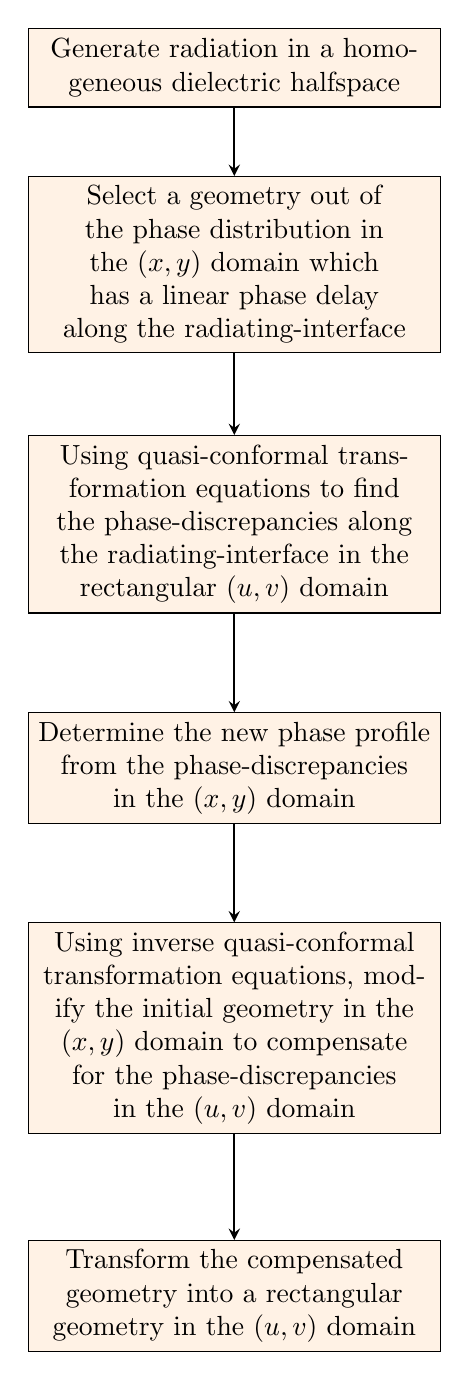
\begin{tikzpicture}[node distance=2cm]

\node (pro1) [rectangle, minimum width=3cm, minimum height=1cm, text centered, text width=5cm, draw=black, fill=orange!10] {Generate radiation in a homogeneous dielectric halfspace};
\node (pro2) [rectangle, minimum width=3cm, minimum height=1cm, text centered, text width=5cm, draw=black, fill=orange!10, below of=pro1, yshift=-.5cm] {Select a geometry out of the phase distribution in the $(x,y)$ domain which has a linear phase delay along the radiating-interface};
\node (pro3) [rectangle, minimum width=3cm, minimum height=1cm, text centered, text width=5cm, draw=black, fill=orange!10, below of=pro2, yshift=-1.3cm] {Using quasi-conformal transformation equations to find the phase-discrepancies along the radiating-interface in the rectangular $(u,v)$ domain};
\node (pro4) [rectangle, minimum width=3cm, minimum height=1cm, text centered, text width=5cm, draw=black, fill=orange!10, below of=pro3, yshift=-1.1cm] {Determine the new phase profile from the phase-discrepancies in the $(x,y)$ domain};
\node (pro5) [rectangle, minimum width=3cm, minimum height=1cm, text centered, text width=5cm, draw=black, fill=orange!10, below of=pro4, yshift=-1.3cm] {Using inverse quasi-conformal transformation equations, modify the initial geometry in the $(x,y)$ domain to compensate for the phase-discrepancies in the $(u,v)$ domain};
\node (pro6) [rectangle, minimum width=3cm, minimum height=1cm, text centered, text width=5cm, draw=black, fill=orange!10, below of=pro5, yshift=-1.4cm] {Transform the compensated geometry into a rectangular geometry in the $(u,v)$ domain};

\draw [thick,->,>=stealth] (pro1) -- (pro2);
\draw [thick,->,>=stealth] (pro2) -- (pro3);
\draw [thick,->,>=stealth] (pro3) -- (pro4);
\draw [thick,->,>=stealth] (pro4) -- (pro5);
\draw [thick,->,>=stealth] (pro5) -- (pro6);

\end{tikzpicture}

\end{center}
\caption{Algorithm of geometric compensation technique.}
\label{fig:flowchart}
\end{figure}